\section{Supplemental}

\subsection{Cram\'er-von Mises Test}

\par Hypothesis testing can be used as an intuitive statistical ground truth for our binned z-scores. Any two distributions can be compared using the Cram\'er-von Mises Test and do not have to be parametric. The null hypothesis is that our z-scores follow a standard normal distribution. Our alternate hypothesis is that our z-scores do not follow a standard normal distribution. If we a p-value of 0.01 for statistical significance, then we reject our null hypothesis. We define OD as the bins where the null hypothesis is rejected and ID otherwise. As we can see from our diffusion data in Figure~\ref{p_values_small}, most data to the left of 0.6 is ID and OD beyond. Our corresponding miscalibration area is shown in Figure~\ref{area_small}.

\begin{figure}[H]
\centering
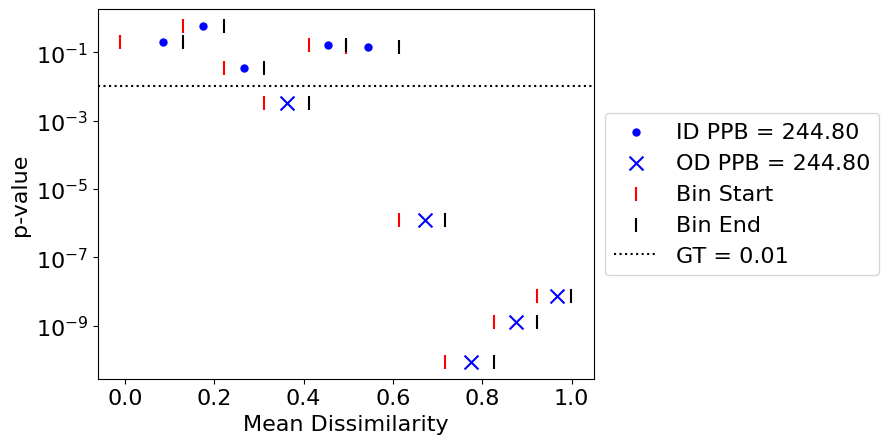
\includegraphics[width=0.95\textwidth]{figures/p_values_small.png}
\caption{PR}
\label{p_values_small}
\end{figure}

\begin{figure}[H]
\centering
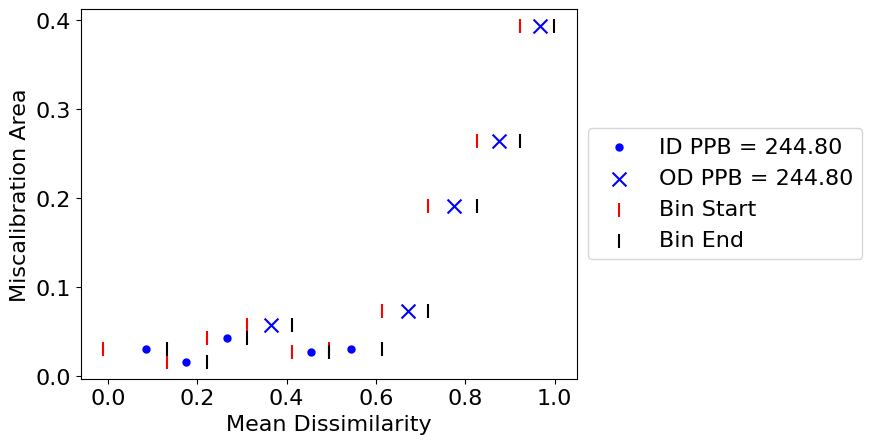
\includegraphics[width=0.95\textwidth]{figures/area_small.png}
\caption{PR}
\label{area_small}
\end{figure}

\par We can increase the number of points per bin and apply Cram\'er-von Mises Test again. We increased the number of points per bin from 244.80 to 1101.60. The p-values are shown in Figure~\ref{p_values_large} and their corresponding miscalibration area are shown in Figure~\ref{area_large}. Although miscalibration areas between Figures~\ref{area_small} and \ref{area_large} do not significantly differ, our p-values from Figures~\ref{p_values_small} and \ref{p_values_large} do change significantly for the second and third bins from the left. This can be attributed to the dependent sampling from our repeated CV. Our methodology of repeatedly splitting our data with K-fold CV and our leave one cluster our CV makes our sampling increasingly dependent.

\begin{figure}[H]
\centering
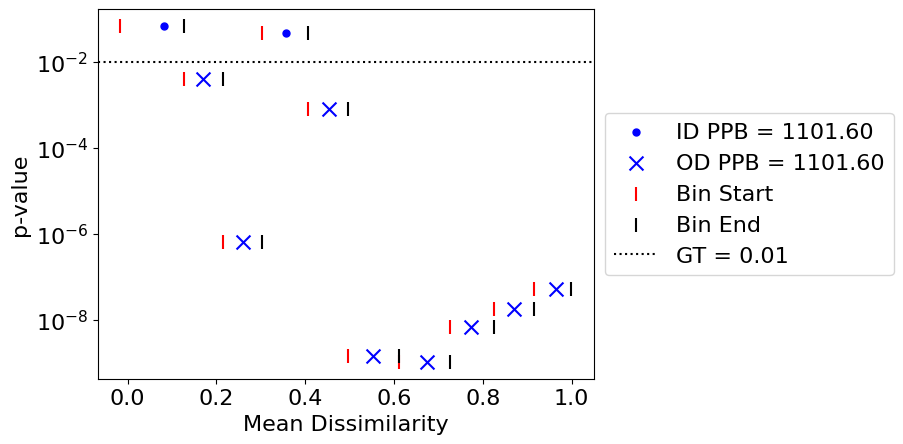
\includegraphics[width=0.95\textwidth]{figures/p_values_large.png}
\caption{PR}
\label{p_values_large}
\end{figure}

\begin{figure}[H]
\centering
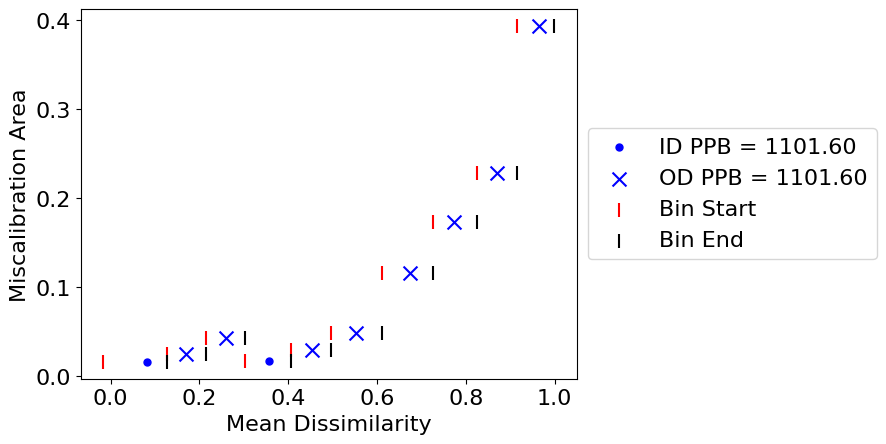
\includegraphics[width=0.95\textwidth]{figures/area_large.png}
\caption{PR}
\label{area_large}
\end{figure}